\documentclass{article}

\usepackage[final,dblblindworkshop]{neurips_2026}
\workshoptitle{2nd Workshop on Advances in Representation Learning for Earth Observation}

\usepackage{amsmath}
\usepackage{booktabs}
\usepackage{graphicx}
\usepackage{microtype}
\usepackage{url}
\usepackage{xcolor}

\pdfinfo{
  /Title (Reusable Change Signal: An Outcome-Blind Audit of Annual Earth Embeddings)
  /Author (Hootan Kamran; Houman Kamran Habibkhani; Atanaz Dorrani)
  /Subject (Annual Earth embeddings and mapped environmental change)
}

\title{Reusable Change Signal: An Outcome-Blind Audit of Annual Earth Embeddings}

\author{%
  \begin{tabular}{@{}c@{\hspace{0.8em}}c@{\hspace{0.8em}}c@{}}
    Hootan Kamran & Houman Kamran Habibkhani & Atanaz Dorrani \\
    \small Northeastern University &
    \small University of the Pacific &
    \small City of Mississauga \\
    {\scriptsize
      \begin{tabular}{c}
        \texttt{h.kamranhabibkhani@}\\[-2pt]
        \texttt{northeastern.edu}
      \end{tabular}} &
    {\scriptsize
      \begin{tabular}{c}
        \texttt{hkamranhabibkhani@}\\[-2pt]
        \texttt{pacific.edu}
      \end{tabular}} &
    {\scriptsize\texttt{a.dorraniarab@gmail.com}}
  \end{tabular}
}

\newcommand{\ECS}{\mathrm{ECS}}

\begin{document}

\maketitle

\begin{abstract}
Precomputed annual Earth embeddings offer a reusable measure of landscape
change without task-specific training. We evaluate whether AlphaEarth
embedding displacement tracks mapped impacts and adds value beyond specialized
optical indices. In an outcome-blind cohort of ten Monitoring Trends in Burn
Severity (MTBS) fires, displacement recovered substantial within-fire severity
ordering (median Spearman $\rho=0.712$), but showed no consistent advantage
over a prespecified Sentinel-2 baseline based on burn-ratio and
vegetation-index change. A second embedding product, TESSERA, showed a
similar pattern. Across eight development cases involving lava emplacement,
forest loss, and drought, AlphaEarth displacement was positively associated
with every mapped reference, although effect sizes varied. These findings
support annual embeddings as portable change representations, though not as
replacements for task-specific measures or operational hazard detectors.
\end{abstract}

\section{Introduction}

AlphaEarth Foundations (AEF) generates annual 64-dimensional embeddings for
10 m pixels across terrestrial and coastal areas, with data available from
2017 to 2025 \citep{brown2025alphaearth,google2025catalog}. Each embedding
summarizes surface conditions and their temporal trajectory at and around a
pixel over a year \citep{brown2025alphaearth}. Year-to-year AEF change can be
measured by comparing the same pixel's embedding across years, but attributing
that change to a specific cause is more difficult for two reasons: (1) annual
embeddings summarize a full year, so short events may be represented alongside
pre- and post-event conditions; and (2) an external map used to explain AEF
changes may be inaccurate in the study area
\citep{comber2012spatial,olofsson2014good} or have little local variation
(e.g., binary extent rather than graded severity) \citep{key2006landscape},
limiting its ability to explain differences in embedding change.

This study addresses two related but distinct questions. First, how closely
does annual AlphaEarth embedding displacement track disturbance patterns shown
in an external reference map? Here, ``track'' refers only to an association
across spatial cells and does not imply disturbance detection, causal
attribution, or ground-truth accuracy. Second, does embedding displacement
provide information beyond changes in conventional spectral indices? The first
question evaluates \textbf{representation fidelity}, meaning how well
AlphaEarth reflects the mapped disturbance pattern, while the second evaluates
its \textbf{incremental value}, or whether it adds information beyond simpler
spectral indices. We contribute (i) an evaluation design that separates
reference-aligned representation fidelity from incremental value over a
task-aligned baseline; (ii) an outcome-blind, frozen AlphaEarth test on ten
MTBS fires; and (iii) an eight-case development audit of the same AlphaEarth
score across lava emplacement, forest loss, and drought. The held-out and
development evidence have distinct roles: the former tests representation
fidelity and added value, while the latter provides preliminary evidence of
reuse without establishing cross-process generalization.

\section{Related work}

Recent work has evaluated geospatial embeddings in different ways. AlphaEarth
has been evaluated across a range of mapping tasks, including classification,
regression, and change detection \citep{brown2025alphaearth}. TESSERA
(Temporal Embeddings of Surface Spectra for Earth Representation and Analysis)
provides open annual 128-dimensional Sentinel-1/2 embeddings and is our direct
representation comparator \citep{feng2026tessera}. NeurEO studies
scale-dependent organization, Rahman environment-aligned coordinates, and
Benavides-Martinez et al.\ task-specific subsets; together, these adjacent
studies establish decodability and redundancy of state embeddings, not
universal process-change axes or added value over process-specific optical
change \citep{vanderplas2025neureo,
rahman2026physicallyinterpretablealphaearthfoundation,benavides2026earth}.
In contrast, we evaluate unsupervised
year-to-year embedding displacement against external disturbance maps, treated
as reference products rather than ground truth.

Our event-specific references are USGS lava extents for Kilauea and Mauna Loa
and CEMS extent for La Palma
\citep{zoeller2020kilauea,cems2021emsr546,zoeller2024maunaloa}, Hansen annual
forest loss \citep{hansen2013forest}, the multi-input U.S. Drought Monitor
\citep{svoboda2002droughtmonitor}, and USFS/USGS MTBS thematic severity,
derived from Landsat imagery and dNBR \citep{eidenshink2007mtbs}.

\section{Method and evaluation protocol}

\paragraph{Annual displacement.}
For model $m$, let $u_{m,p}^{(y)}$ denote its unit-normalized annual embedding
at pixel $p$ in year $y$; we compute
\[
d_{m,p}^2=\lVert u_{m,p}^{(\mathrm{post})}
-u_{m,p}^{(\mathrm{pre})}\rVert_2^2
=2-2\cos(u_{m,p}^{(\mathrm{post})},u_{m,p}^{(\mathrm{pre})}).
\]
These values are averaged within H3 hexagonal grid cells \citep{h3spec}; we
call the resulting AlphaEarth quantity embedding change squared (ECS). ECS is
a descriptive measure of change magnitude and is not intended as a hazard
detector. Our representation comparator, TESSERA v1.0 (vultr manifest),
provides int8 vectors that are dequantized and $l_2$-normalized per pixel
before the same displacement and H3 averaging on the frozen fire cells.
Because model scales are not directly comparable, each model's displacement
is instead correlated by Spearman rank with the same event reference;
cross-model comparisons use those within-fire coefficients.

\paragraph{Outcome-blind held-out MTBS fire test.}
MTBS analysts derive dNBR from pre- and post-fire Landsat imagery and interpret
it with the imagery, ecological context, ancillary evidence, and, where
available, field observations such as Composite Burn Index plots to set
event-specific severity thresholds
\citep{eidenshink2007mtbs,picotte2020mtbs}. We therefore use MTBS as the
study's standardized cohort-wide burn-severity reference. Before AlphaEarth
access, a frozen metadata snapshot deterministically selected ten U.S. fires
plus ordered reserves across years, regions, sizes, and dominant land-cover
strata. Official boundaries and 30\,m MTBS thematic rasters define the
reference within each H3-r8 cell (resolution 8, ${\sim}0.74\,\mathrm{km}^2$
mean area) as the fraction of classes 3--4 (moderate/high severity) among
classes 1--5.\footnote{MTBS thematic classes: 1 unburned to low, 2 low,
3 moderate, 4 high severity, 5 increased greenness
\citep{eidenshink2007mtbs}.} Class 2 is valid low severity, contributing to
the denominator but not the numerator. Background/NoData and non-processing
areas are excluded \citep{eidenshink2007mtbs}. Cell centers must lie within
the event boundary, at least 80\% of each cell must have valid MTBS support,
and at least 200 cells must remain. The exact H3 population is frozen before
AlphaEarth extraction. Four County had a constant target and, before
AlphaEarth access, was replaced by the next prespecified reserve, Walker.

For an event in year $y$, AlphaEarth, TESSERA, and Sentinel-2 use full calendar
years $y-1$ and $y+1$. The optical comparator median-composites cloud-masked
\texttt{S2\_SR\_HARMONIZED} reflectance \citep{esa2021sentinel2} and computes
two spectral indices, dNBR and dNDVI, per H3 cell, with positive values
indicating post-event decrease (Appendix~\ref{app:s2}).

\paragraph{Event-level estimands.}
Within-event Spearman correlation ($\rho$) summarizes representation fidelity:
whether embedding displacement recovers MTBS-aligned severity ordering. It is
not an equivalence criterion. For fire $e$, the frozen primary statistic is
\[
\Delta_e^{\mathrm{A}}=\rho(\ECS,\mathrm{MTBS})
-\max\{\rho(\mathrm{dNBR},\mathrm{MTBS}),
\rho(\mathrm{dNDVI},\mathrm{MTBS})\}.
\]
This statistic measures standalone advantage and does not assess whether
displacement complements the optical indices. The prespecified
$\Delta_e^{\mathrm{T}}$ substitutes normalized TESSERA displacement on the
same frozen cells. We report unweighted event means and 95\% percentile
intervals from 100,000 event-bootstrap resamples. Each fire, not its
autocorrelated H3 cells, is one inferential unit \citep{clifford1989spatial};
no cell-level $p$-values are used. Selecting the stronger of dNBR and dNDVI
deliberately favors the optical baseline; the directional alternative is
$\bar{\Delta}^{\mathrm{A}}>0$. Spearman association is primary because the
MTBS target derives from thematic classes. All correlations rank severity
within official perimeters, with no unaffected outside-perimeter cells.

\paragraph{Development audit and temporal support.}
Mean ECS and reference values are reduced to predefined H3 cells; only finite
cells valid in both layers are retained. Each eruption is bracketed by the
preceding and following annual embeddings: $2017\rightarrow2019$ for Kilauea,
$2020\rightarrow2022$ for La Palma, and $2021\rightarrow2023$ for Mauna Loa.
Lava support uses WorldCover non-water pixels plus mapped lava; La Palma also
restricts non-lava support to the CEMS analyzed footprint
\citep{zanaga2021worldcover}. Two 2021 forest comparisons multiply Hansen
\texttt{lossyear} indicators by year-2000 canopy cover. Three drought
comparisons use absolute change between fixed April--October mean USDM scores,
avoiding event-specific peak-month selection. We score weekly USDM categories
as none $=0$ and D0--D4 $=1$--$5$; absolute change treats intensification and
recovery alike. Development cases were not screened by correlation magnitude
or sign.

\section{Results}

\begin{figure*}[t!]
  \centering
  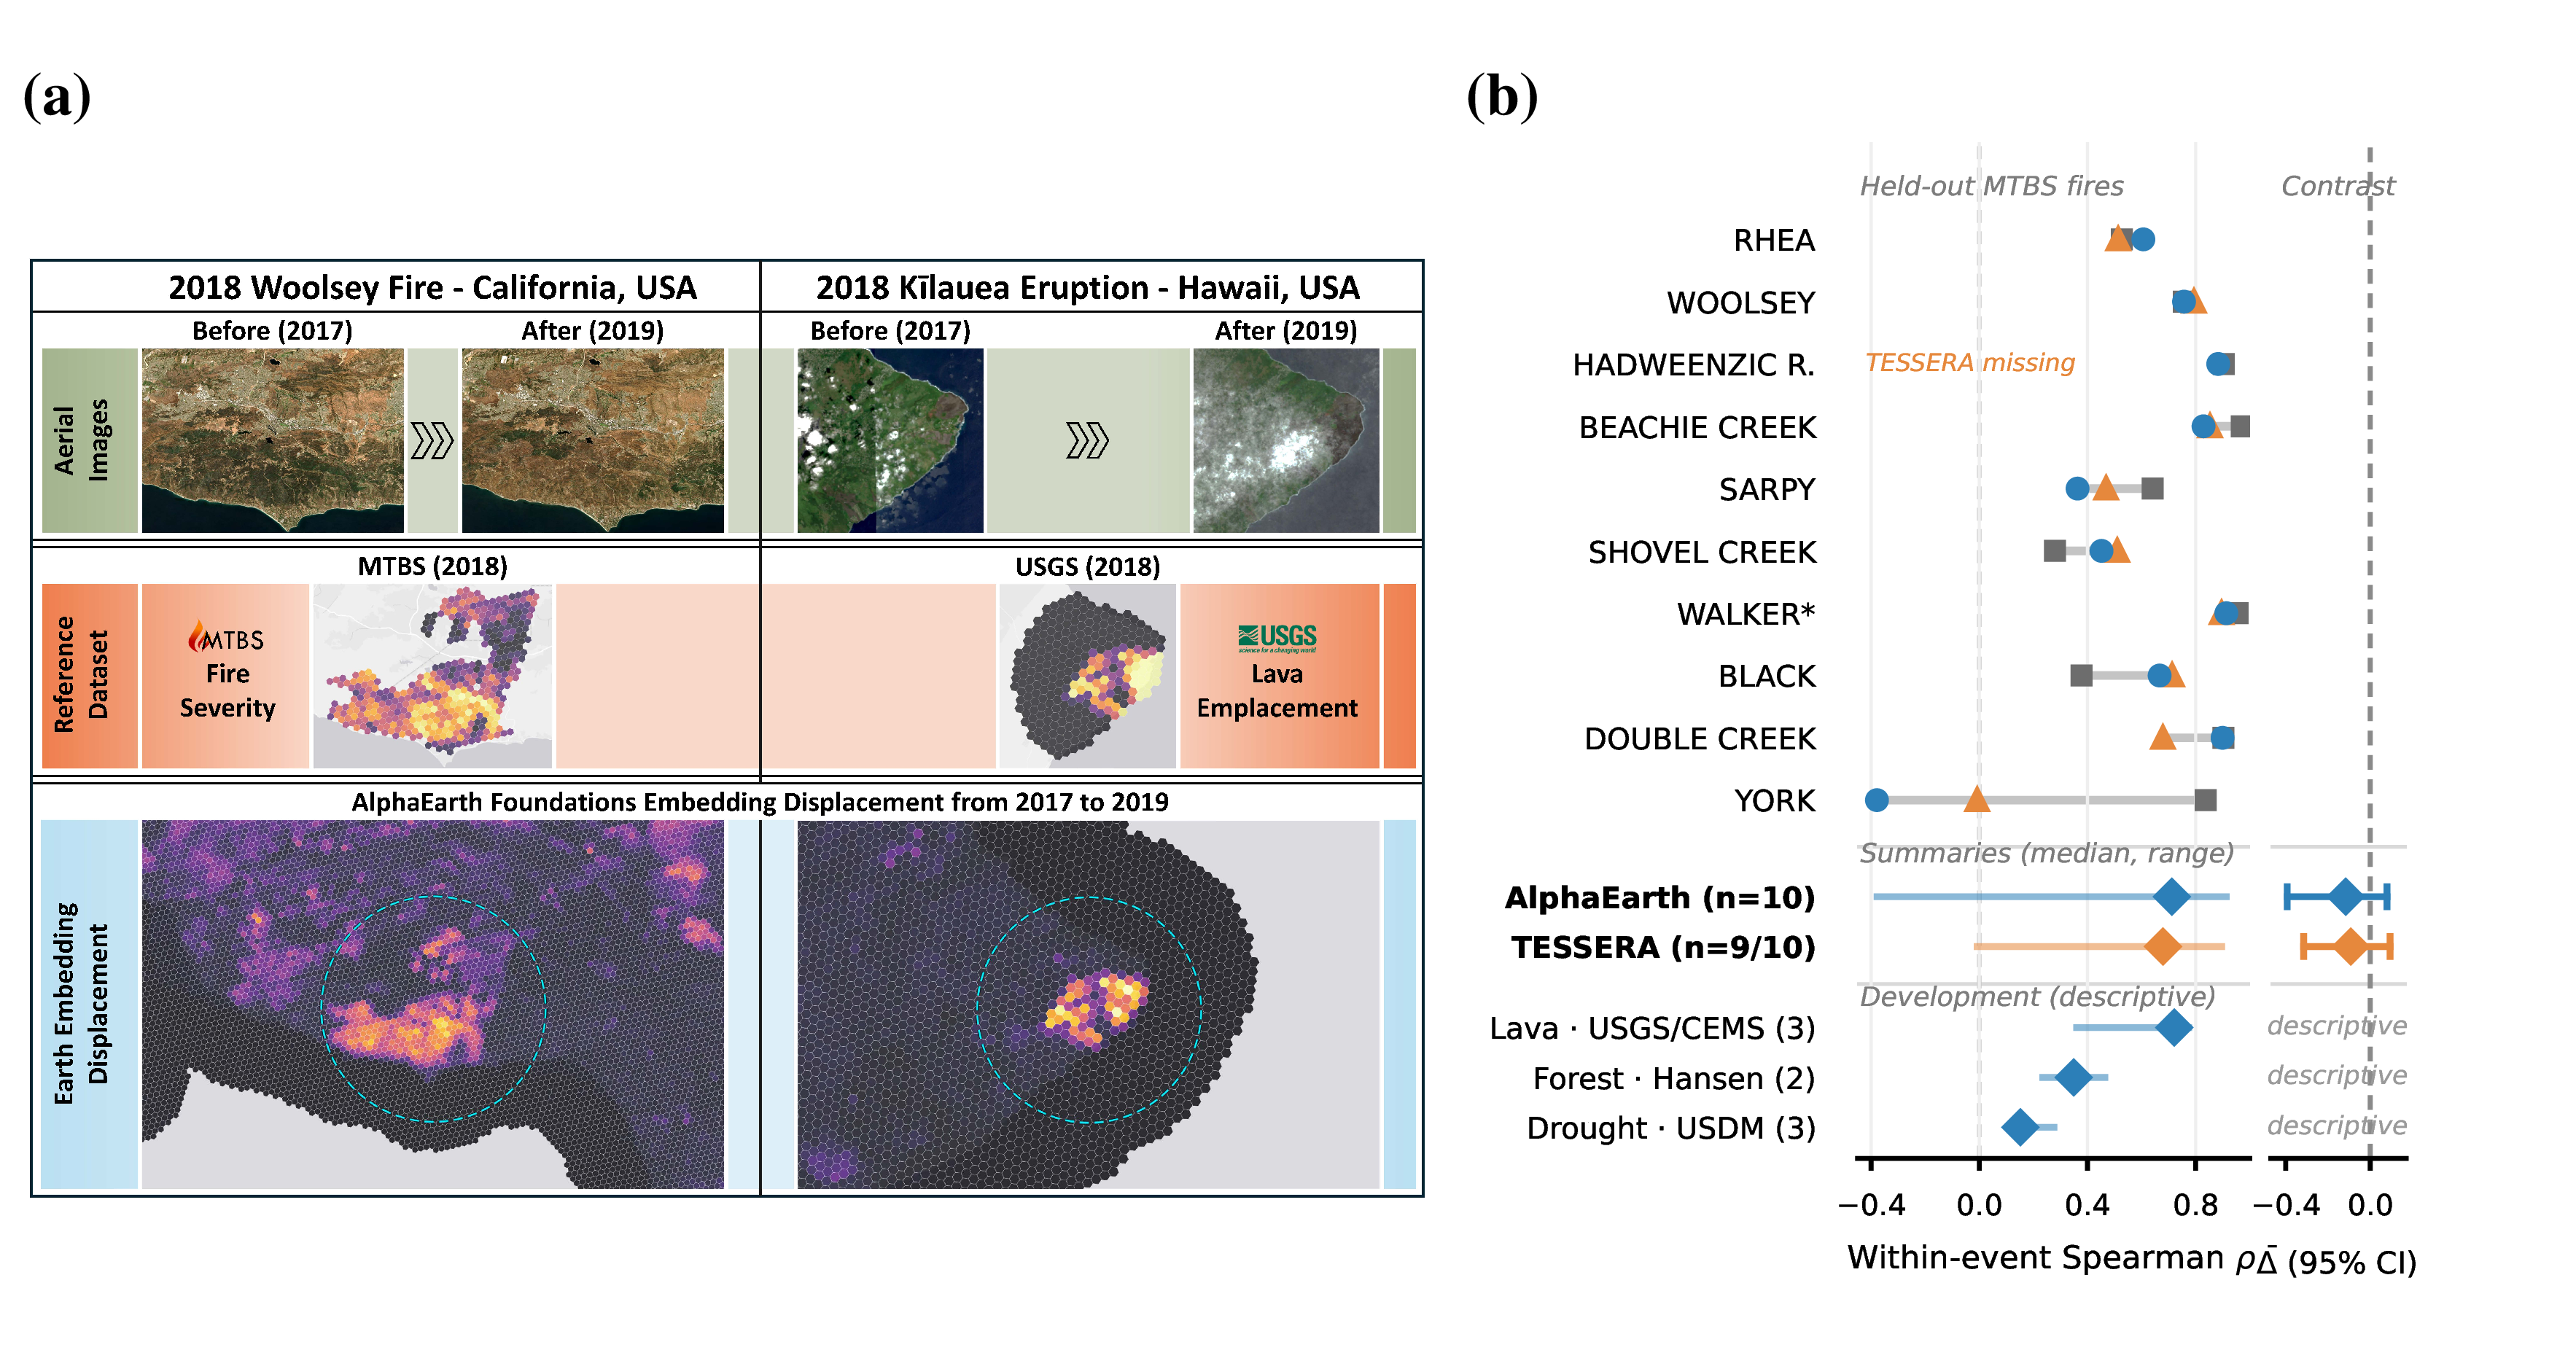
\includegraphics[width=\linewidth]{figure_primary.png}
  \caption{\textbf{Fidelity illustration and frozen evidence summary.}
  (a) One held-out fire and one development case, both 2018 events with
  displacement bracketed $2017 \to 2019$: the Woolsey Fire against MTBS
  severity (within-event $\rho=0.757$) and the Kilauea eruption against USGS
  lava extent (within-event $\rho=0.774$). Rows show before/after imagery,
  the official reference on the common H3 grid, and AlphaEarth displacement
  (ECS). Each official reference is task-specific, whereas the AlphaEarth
  displacement shown is the same unsupervised score in both cases---and in
  every case of panel~(b). (b) Graphical summary of
  Table~\ref{tab:results} (Appendix~\ref{app:evidence}): per-event
  associations for the ten held-out fires (blue circles AlphaEarth, gray
  squares best-of-two optical, orange triangles TESSERA; Walker* is the
  prespecified reserve; one official TESSERA year tile is missing), model and
  development-family summaries (diamonds medians, lines ranges), and mean
  incremental contrasts with 95\% event-bootstrap intervals (dashed line at
  zero). Map colors are normalized per panel.}
  \label{fig:primary}
\end{figure*}

\paragraph{Held-out fidelity and incremental value.}
A simple AlphaEarth displacement score recovered substantial but heterogeneous
MTBS-aligned severity ordering (Figure~\ref{fig:primary}). Nine of ten fires
had positive associations, with median $\rho=0.712$ (exact two-sided
event-level sign test, $p=0.021$). AlphaEarth exceeded the optical comparator
in four of ten. The frozen mean endpoint was
$\bar{\Delta}^{\mathrm{A}}=-0.116$ (95\% interval $[-0.393,0.079]$); median
$\Delta_e^{\mathrm{A}}=-0.012$. Thus, the study supports representation
fidelity but establishes superiority for neither AlphaEarth nor the optical
comparator. The secondary analysis with the representation comparator,
TESSERA, was prespecified on the frozen fire populations. Nine events were
evaluable; the official v1.0 (vultr) manifest lacked one required year--tile
object for the tenth, which remained in the AlphaEarth cohort as
TESSERA-missing. TESSERA exceeded the optical comparator in three of nine
events; $\bar{\Delta}^{\mathrm{T}}=-0.092$ (95\% interval
$[-0.315,0.094]$). The descriptive paired mean AlphaEarth-minus-TESSERA
$\rho$ difference was $-0.034$ (95\% interval $[-0.138,0.059]$). Neither
interval establishes a consistent advantage.

\paragraph{Development evidence.}
The family summaries include all predefined cases without outcome screening.
All eight associations are positive, with family medians of $0.721$ (lava),
$0.349$ (forest loss), and $0.152$ (drought)
(Table~\ref{tab:results}, Appendix~\ref{app:evidence}), providing early
evidence that the same unsupervised change score may be reusable across
distinct environmental processes. Post hoc spatial sensitivity remained
positive at the primary block scale in all eight cases but mixed or
unassessable at coarser scales (Appendix~\ref{app:spatial}). These
heterogeneous development cases do not establish general cross-process
performance or a family-level effect.

These analyses evaluate direct reuse of precomputed displacement; we did not
measure label efficiency or train downstream models. Whether displacement adds
information conditional on the optical indices, for example, through partial
rank correlation on the frozen cells, is the natural next analysis and was not
prespecified here. Precomputed embeddings supply one change representation
that transfers across processes, whereas the matched optical indices remained
competitive within the fire cohort; we therefore read the cross-process
results as evidence of portability rather than of task-level advantage.

\section{Validity, omissions, and limitations}

The development audit is deliberately heterogeneous and cannot estimate a
population-level effect. Only the fire cohort was selected outcome-blind and
held out before AlphaEarth extraction, and ten events give a wide bootstrap
interval. One retained event (YORK) has
$\Delta_e^{\mathrm{A}}=-1.215$; omitting it would give a descriptive mean of
$0.006$. We retain the event and keep the frozen endpoint unchanged
(Appendix~\ref{app:york}). The MTBS comparison is not independent optical
validation: analysts derive thematic classes largely by thresholding Landsat
dNBR, with interpretation and occasional ancillary evidence
\citep{eidenshink2007mtbs}. Our Sentinel-2 dNBR is not the same image product,
but it targets the same spectral construct. We therefore interpret
within-event $\rho$ as criterion-aligned fidelity, and
$\bar{\Delta}^{\mathrm{A}}$ and $\bar{\Delta}^{\mathrm{T}}$ as added value
relative to a product-aligned baseline, not as a general
embedding-versus-imagery verdict.

External maps have omissions and class semantics; valid-support exclusion
changes the target population; and annual embeddings may respond to phenology,
management, sensor/compositing effects, or unrelated change. H3 averaging
smooths sub-cell structure. Because MTBS cells are sampled only inside mapped
perimeters, the study ranks severity within them and does not address fire
detection, localization, or behavior on unaffected landscapes. Artifact and
replay details appear in Appendix~\ref{app:reproducibility}.

\section{Conclusion}

A simple difference between readily available annual embeddings recovered
substantial MTBS-aligned severity ordering in most held-out fires, with no
consistent standalone advantage over target-aligned spectral indices for
either AlphaEarth or TESSERA. Positive but variable development associations
across lava emplacement, forest loss, and drought support annual embeddings as
broadly reusable sources of mapped-change information; on this evidence they
do not replace specialized indices or operational hazard detectors.

\clearpage
\bibliographystyle{plainnat}
\bibliography{references}

\clearpage
\appendix

\section{Frozen evidence summary}
\label{app:evidence}

\begin{table}[ht]
  \caption{Frozen evidence summary. Median $\rho$ summarizes representation
  fidelity. Held-out contrasts compare each embedding with the prespecified
  best-of-two optical comparator, then average equally over events. Intervals
  resample events. Development rows summarize predefined non-fire cases by
  family.}
  \label{tab:results}
  \centering
  \footnotesize
  \setlength{\tabcolsep}{4.0pt}
  \begin{tabular}{@{}llrrl@{}}
    \toprule
    Study & Reference & Events & Fidelity: median $\rho$ (range) &
    Incremental contrast (95\% interval) \\
    \midrule
    AlphaEarth held-out
      & MTBS severity
      & 10
      & $0.712$ ($-0.378,0.913$)
      & $\bar{\Delta}^{\mathrm{A}}=-0.116$ ($-0.393,0.079$) \\
    TESSERA secondary
      & MTBS severity
      & 9/10
      & $0.679$ ($-0.008,0.896$)
      & $\bar{\Delta}^{\mathrm{T}}=-0.092$ ($-0.315,0.094$) \\
    Lava development
      & USGS/CEMS extent
      & 3
      & $0.721$ ($0.360,0.774$)
      & descriptive \\
    Forest development
      & Hansen loss
      & 2
      & $0.349$ ($0.235,0.464$)
      & descriptive \\
    Drought development
      & USDM change
      & 3
      & $0.152$ ($0.126,0.276$)
      & descriptive \\
    \bottomrule
  \end{tabular}
\end{table}

\section{Sentinel-2 comparator details}
\label{app:s2}

B4 (red), B8 (near-infrared), and B12 (shortwave infrared) are
median-composited after filtering scenes to at most 70\% reported cloud cover
and masking cloud, shadow, cirrus, snow, and invalid pixels; each pixel
requires at least two clear observations per year. NDVI summarizes
near-infrared/red vegetation contrast, while NBR uses
near-infrared/shortwave-infrared contrast sensitive to burn and moisture
change. We define
$\mathrm{NDVI}=(B8-B4)/(B8+B4)$,
$\mathrm{NBR}=(B8-B12)/(B8+B12)$,
$\mathrm{dNBR}=\mathrm{NBR}_{\mathrm{pre}}-\mathrm{NBR}_{\mathrm{post}}$, and
$\mathrm{dNDVI}=\mathrm{NDVI}_{\mathrm{pre}}-\mathrm{NDVI}_{\mathrm{post}}$.
Positive values indicate post-event decreases. Both indices are averaged over
valid pixels within each H3-r8 cell.

\section{Spatial-sensitivity details}
\label{app:spatial}

A frozen post hoc spatial sensitivity retained positive primary-scale block
correlations in all eight cases (equal-event median Spearman correlation
$0.424$); five passed Holm-adjusted block-label permutation tests, while
coarsest-scale results were mixed or unassessable in six cases. Free
block-label permutation does not guarantee exchangeability across broad
spatial gradients; this sensitivity is supplementary and scale-dependent.
Because these are heterogeneous development cases, they do not establish
general cross-process performance or a family-level effect.

\section{YORK target diagnostic}
\label{app:york}

The ten AlphaEarth coefficients span $-0.378$ to $0.913$ over 6,864 frozen
event-cells. YORK (2023, Mojave shrub/sparse; $n=410$) passed every QA gate but
has $\rho_{\rm ECS}=-0.378$ for the frozen moderate/high target. A labeled post
hoc diagnostic found that 84.0\% of mapped pixels were MTBS class 2: ECS was
near zero for an ordinal target ($\rho=-0.038$) but positive for any-severity
fraction ($\rho=0.344$), while remaining below matched optical change in both.
This is consistent with sensitivity to low-severity extent rather than
severity ordering; the frozen endpoint is unchanged.

\section{Reproducibility}
\label{app:reproducibility}

The artifact includes canonical pre-outcome protocols and hashes, failed
attempts and reserve ordering, immutable H3 populations, per-event metrics,
official-reference replay, and code for the event bootstrap. All weak,
negative, and missing cases are retained. The artifact is available at
\url{https://github.com/whotank/alphaearth-disaster-pipeline}.

\end{document}
